\documentclass[10pt,a4paper]{report}
\usepackage[utf8]{inputenc}
\usepackage[french]{babel}
\usepackage{amsmath,amsfonts,amssymb}
\usepackage{graphicx}
\usepackage{caption}
\usepackage{systeme}

\begin{document}
\title{Détermination expérimentale de la conductivité thermique des semi-conducteurs}
\author{Leo-Paul BAUDET,  Alexandre CORRIOU, Noah VEYTIZOUX, \\Evan VOYLES, Stefan GA\L KIEWICZ \\sous l'encadrement de
Dr. Mohamed Boutchich}
\maketitle
\tableofcontents
\chapter{Introduction}
Les semis-conducteurs sont utilisés dans une variété d'applications. Par exemple, dans les télécommunications à fibre optique qui ont été développées à un rythme croissant depuis maintenant plus de 20 ans. Les progrès réalisés ces dernières décades dans ce domaine peuvent être mesurés en remarquant que les premières liaisons optiques trans-océaniques pouvaient transmettre jusqu'à 80.000 conversations téléphoniques simultanées alors que les premiers câbles coaxiaux trans-océaniques voyaient leur capacité de transmission saturer à 36 voix simultanées. Cette progression est le résultat de nombreux efforts de développement de la technologie des fibres optiques et des dispositifs électro-optiques semi-conducteurs : les diodes électroluminescentes, les photodiodes et surtout les lasers à semi-conducteurs. De manière générale, l’industrie des circuits et des composants électroniques à semi-conducteurs est à la base du développement d’un grand nombre de technologies modernes parmi lesquelles se trouvent l’informatique, les télécommunications, le traitement de l'information et l’automatique. Cette industrie est basée sur deux concepts : la miniaturisation et la gravure des composants semi-conducteurs. La miniaturisation est rendue possible par le fait que les vecteurs d’information sont des particules élémentaires : les électrons. Les circuits et les composants étant essentiellement à géométrie planaire à l’heure actuelle, leur reproduction à grande échelle à été rendue possible grâce aux procédés classiques de gravure transposés aux échelles micrométriques. Les composants électroniques mettent donc à profit les propriétés dynamiques des électrons dans les semi-conducteurs. Il faut donc, pour tenter de comprendre le fonctionnement de ces composants, préciser leur propriétés et définir les grandeurs physiques dont les évolutions conditionnent les propriétés électriques ou optiques de ces composants. L'objectif de notre travail s'inscrit donc dans cette dynamique puisqu'il s'agit de réussir à déterminer expérimentalement la conductivité thermique de semis-conducteurs.

\chapter{Définitions préliminaires}
\section{Conducteurs, isolants et Semi-conducteurs}
Parmis la multitude de materiaux existants  on distingue trois grand types de matériaux.
Les  matériaux  ayant  la  plus  faible  résistivité  à  température  ambiante,  typiquement inférieure  à  $10^{-5} \Omega$m,  sont  les  métaux  (cuivre,  or,  argent,  aluminium...). Leur bonne  conduction électrique provient essentiellement du fait que ces éléments possèdent une faible electronégativité. En effet, au sein des cristaux métalliques, les liaisons que réalisent les atomes du réseau cristallin entre eux ne sont plus des liaisons covalentes (liaisons localisées) mais des liaisons métalliques (liaisons délocalisées). Cela s'explique par le fait que les électrons de leur couche de Valence ne sont pas contraint à "rester" proche du noyau mais sont libre de se déplacer dans le cristal de part la faible électronegativité des atomes constituant celui ci. Ces électrons sont alors appelés électrons libres. Ainsi, lorsque l'on applique une différence de potentiel sur un cristal métallique, les électrons libres crées alors eux même une différence de potentiel au sein de celui ci d'où la bonne conductivité des cristaux métalliques. Enfin, une augmentation de  la
température provoque une légère augmentation de la résistivité, pouvant s’expliquer par le fait que les électrons libres sont gênés dans leur déplacement par leurs vibrations.

 Les  matériaux  dont  la  résistivité  est  typiquement  supérieure  à  $10^8 \Omega$m  sont  considérés comme isolants ; c’est le cas pour le verre, le mica, la silice (SiO2), le carbone (diamant). Cette fois ci, les atomes constituants ces cristaux (cristaux covalents) sont des atomes très électronégatifs qui, pour les même raisons citées ci dessus réalisent alors  des liaisons covalentes qui sont des liaisons localisées. Ainsi, les électrons de la couche de Valence ne son plus libres et lorsque qu'on applique une différence de potentiel sur un cristal covalent, cette fois ci, aucune différence de potentiel n'est crée au sein du cristal, ils ne conduisent donc pas bien le courant. Ici, l’augmentation  de  la  température  peut  provoquer  la  libération  d’électrons  (ainsi  que  de "trous")  qui  peuvent  participer  à  la  conduction  électrique,  ce  qui  provoque  une  baisse  de  la résistivité avec la température.

Entre  les  métaux  et  les  isolants  se  trouvent  les  semi-conducteurs  dont  la  résistivité
varie de $10^{-3} à 10^4 \Omega$m. La conduction électrique se fait par les électrons et les trous. Un semi-conducteur peut être soit pur auquel cas il est dit intrinsèque, soit dopé par des impuretés (qui permettent de contrôler sa résistivité) auquel cas il est dit extrinsèque. Si on prend, par exemple, du Silicium pur  et  qu’on  lui  ajoute  un  atome  de  Bore  ou  de Phosphore,  sa résistivité passe de$ 10^3 \Omega$m à environ $10^-2 \Omega$m.
\newline
\begin{center}
\begin{tabular}{|l|p{3cm}|c|p{3cm}|}\hline
colonne tableau périodique & semi-conducteurs\\\hline
IV & Ge, Si\\\hline
III-V & GaAs, GaP, GaSb, InAs, InSb, InP\\\hline
II-VI & CdS, HgTe, CdTe, ZnTe, ZnS \\\hline
\end{tabular}
\end{center}
\begin{center}
Tableau 1.1: Exemples de semi-conducteurs
\end{center}
\section{Grandeurs thermodynamiques}
\subsection{Puissance}
La puissance correspond à la dérivée de l'énergie FOURNIE par rapport au temps:
\newline
\begin{center}
{$P=\frac{dQ}{dt}$}
\end{center}
En thermodynamique, l’énergie fournie est un transfert thermique que l'on note Q
\subsection{Coefficient de température d'une résistance}
 C’est un coefficient qui rend compte du fait qu’un conducteur ohmique (résistance) ne possède pas la même résistance à différentes températures, il permet alors de définir la résistance d’un conducteur ohmique quelque soit la température (il est en ohm par kelvin) :
\newline
\begin{center}
\begin{equation}
R=R_{0}(1+\alpha(T-T_{0}))
\end{equation}
\end{center}
\begin{center}
avec $R_{0}$ la résistance à $T_{0}$
\end{center}
\subsection{Conductivité thermique}
C’est une grandeur qui rend compte de la capacité d’un matériaux à transmettre plus ou moins bien de la chaleur
\subsection{Flux thermique}
Intuitivement, c’est la quantité d’énergie thermique qui passe par unité de temps à travers une surface donnée (il est donc en J/s=W). Il est commode de le voir comme une grandeur « globale » ; qui décrit globalement la quantité d’énergie qui passe dans une surface. On le défini de la manière suivante :
\begin{center}
\begin{equation}
\Phi_{th}=\frac{\delta Q}{dt}
\end{equation}
\end{center}
\subsection{Vecteur densité de flux thermique}
Il représente en chaque point d'une surface donnée la quantité d’énergie qui y passe (il est donc en J/(sm²)) Il est commode de le voir comme une grandeur locale; le sens de ce vecteur correspond au sens du transfert et sa norme à la quantité d'énergie transmise en son point d'application. Il est relié au flux par la formule suivante :
\begin{center}
\begin{equation}
\Phi_{th}=\iint_{S} \vec{j_{th}} \,d\vec{S}
\end{equation}
\end{center}
\begin{center}
avec S une surface
\end{center}
Dans d’autres domaines physique, on retrouve des grandeurs analogues au flux et à ce vecteur comme en électromagnétisme avec le vecteur densité volumique de charge et le flux d’un champ électrique, en électrocinétique avec l’intensité et le vecteur densité volumique de courant.
\newline
Par ailleurs, ce vecteur est relié à la température par la loi de Fourier :
\begin{center}
\begin{equation}
\vec{j_{th}}=-\lambda\vec{\nabla}T(M,t)
\end{equation}
avec
\begin{equation}
 \vec{\nabla}T(M,t)=\frac{\partial T(M,t)}{\partial x}\vec{e_{x}}+\frac{\partial T(M,t)}{\partial y}\vec{e_{y}}+\frac{\partial T(M,t)}{\partial z}\vec{e_{z}}
\end{equation}
et $\lambda$ la conductivité thermique
\end{center}
Cette loi rend simplement compte qu'un transfert thermique est d’autant plus important que la conductivité est forte ou que la variation de la température est forte
\chapter{Méthode 3$\omega$}
\section{Cadre d'étude}
L’objectif est de réussir à déterminer expérimentalement la conductivité thermique de semi-conducteurs. La difficulté est que les semi-conducteurs utilisés sont pour la plupart très fins, et les méthodes classiques de détermination de conductivité thermique (pour les solides de tailles « normale ») ne sont plus applicables directement. Il faut donc trouver une méthode qui permette de contourner ce problème. Tout d’abord, il s’agit de se ramener à un solide de taille « normal » dont on saura alors caractériser plus facilement la conductivité thermique. Pour cela, on va superposer le semi-conducteur sur un substrat (dont on connait la conductivité) suffisamment épais et on fixera au sein du semi-conducteur une résistance (ou un fil) qui par effet joule permettra de délivrer une onde de chaleur dans le semi-conducteur. Parmi les différentes méthode 3$\omega$ existantes, nous allons utiliser celle dite différentielle qui consiste à caractériser le substrat seul puis l’ensemble substrat + couches minces. Pour les caractériser, il « suffit » de tracer les variations de températures en fonction de la fréquence du courant injecté. L'approche différentielle consiste alors à comparer les courbes expérimentales des échantillons comprenant les couches minces à celle obtenue avec le substrat seul de manière à estimer la résistance thermique introduite par les couches minces.
\section{Etude du substrat seul infini}
\subsection{Détermination de l'oscillation en température}
Le principe est d’utiliser le même élément à la fois pour perturber thermiquement le système et pour mesurer les variations de température en un point du système. On injecte dans l’échantillon un courant sinusoïdal de pulsation $\omega$ à travers un fil chauffant (joue le rôle d’une résistance)
\begin{center}
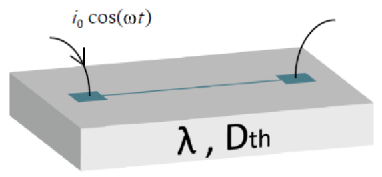
\includegraphics[scale=0.5]{../schéma et graphes/substratbisbis.png}
\captionof{figure}{Schema substrat}
\label{fig1}
\end{center}
La résistance R de ce fil, de coefficient de température $\alpha$, n’est pas constante au cours du temps puisque sa température varie ; la valeur de sa résistance est donc donné par :
\begin{center}
\begin{equation}
R=R_{0}(1+\alpha(T-T_{0}))
\end{equation}
\end{center}
Par effet Joule, la puissance dissipée par le fil aura une fréquence deux fois plus élevée que le courant injecté et se composera d’une partie constante (notée dc) ainsi que d’une partie alternative (notée ac)
\begin{center}
\begin{equation}
P=R*I^2=\frac{R*i_{0}^2}{2}(1+cos(2\omega t))=P_{ac}+P_{dc}
\end{equation}
\end{center}
On voit alors clairement que la puissance va osciller deux fois plus rapidement. Et donc Q va également osciller à la pulsation 2$\omega$, donc le flux thermique aussi, donc le vecteur densité de flux thermique aussi ; donc la température aussi. En résumé, l’oscillation de la puissance va créer des ondes de températures qui varient à la même fréquence que P mais pas à la même phase. Ce déphasage est lié à la conduction thermique dans le substrat. On obtient alors la formule suivante pour la variation de température au cours du temps en un point donné du solide :
\begin{center}
\begin{equation}
\Delta T=\Delta T_{dc}+\Delta T_{ac}=\Delta T_{dc}+\lvert \Delta T_{ac} \rvert cos(2\omega t+\phi)
\end{equation}
$\lvert \Delta T_{ac} \rvert$ designe l’amplitude de la température alternative.
L’amplitude de la température alternative et son déphasage dépendent évidemment des propriétés thermophysiques de l’échantillon (en particulier de sa conductivité thermique).
\end{center}
Partant de l’expression de la résistance exprimée précédemment et de la relation trouvée pour la température, on obtient l’expression suivante :
\begin{center}
\begin{equation}
R=R_{0}(1+\alpha \Delta T_{dc})+R_{0}(\alpha \lvert \Delta T_{ac} \rvert cos(2\omega t+\phi)
\end{equation}
\begin{equation}
R=R_{dc}+R_{ac}cos(2\omega t+\phi)
\end{equation}
où $\Delta T_{dc}=T_{dc}-T_{0}$ est l'élévation de température par rapport à la température ambiante
\end{center}
La résistance du fil va donc osciller autour d’une résistance $R_{dc}$ à la même fréquence que la température. En mesurant la tension aux bornes de cette résistance selon la loi d’Ohm, une composante oscillant à la fréquence 3$\omega$ apparaît :
\begin{center}
\begin{equation}
V=R*I=(R_{dc}+R_{ac}cos(2\omega t+\phi))*I_{0}cos(\omega t)
\end{equation}
\begin{equation}
V=V_{1\omega}cos(\omega t)+V'_{1\omega}cos(\omega t+\phi)+V_{3\omega}cos(3\omega t+\phi)
\end{equation}
avec
\begin{equation}
V_{1\omega}=I_{0}R_{0}(1+\alpha \Delta T_{dc})
\end{equation}
\begin{equation}
V'_{1\omega}=I_{0}R_{0}(\frac{1}{2}\alpha \lvert \Delta T_{ac} \rvert)
\end{equation}
\begin{equation}
V_{3\omega}=I_{0}R_{0}(\frac{1}{2}\alpha \lvert \Delta T_{ac} \rvert)
\end{equation}
\end{center}
\subsection{Equation de la chaleur}
\begin{center}
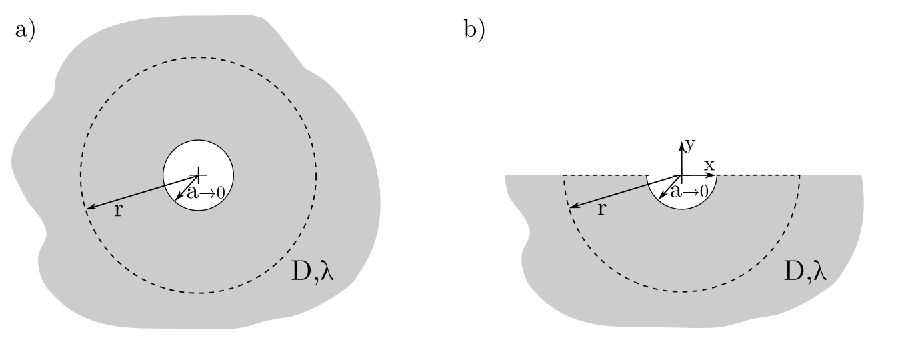
\includegraphics[scale=0.5]{../schéma et graphes/schema.png}
\captionof{figure}{Schemas décrivant les modèles thermiques (vue en coupe)}
\label{fig2}
\end{center}
Si le milieu est supposé infini, l’équation de la chaleur s’obtient en se plaçant en coordonnées cylindriques compte tenu de la géométrie du problème, on obtient:
\begin{center}
\begin{equation}
\frac{\partial T(r,t)}{\partial t}=D\frac{1}{r}(r\frac{\partial T(r,t)}{\partial r})
\end{equation}
avec D la diffusivité thermique
\end{center}
Par ailleurs, d'après la formule (3.3), on peut écrire:
\begin{center}
\begin{equation}
T(r,t)=T_{0}+\Delta T_{dc}(r)+\Delta T_{ac}(r,t)
\end{equation}
où $\Delta T_{dc}(r)=T_{dc}(r)-T_{0}$
\end{center}
En combinant ces deux équations, on obtient alors:
\begin{center}
\begin{equation}
\frac{1}{D}(\frac{\partial \Delta T_{ac}(r,t)}{\partial t})-\frac{1}{r}\frac{\partial}{\partial r}(r\frac{\Delta T_{ac}(r,t)}{\partial r})=\frac{1}{r}\frac{\partial}{\partial r}(r\frac{\Delta T_{dc}(r)}{\partial r})=0
\end{equation}
\end{center}
Le problème revient donc à résoudre l’équation de la chaleur pour $\Delta T_{ac}$. La source de chaleur sera assimilée dans un premier temps à un cylindre de longueur l et de rayon a. On établira une équation dans la limite où le rayon a tend vers 0 permettant de s’approcher du modèle de ligne de chauffe”. On a alors les conditions aux limites suivantes:
\begin{center}
\begin{equation}
\systeme{-\lim\limits_{a \rightarrow 0}2\lambda\pi a\frac{\partial \Delta T_{ac}(r,t)}{\partial r}=Q(r;t),\lim\limits_{r \rightarrow +\infty}\Delta T_{ac}(r;t)=0}
\end{equation}
où Q(r,t) est la puissance injectée dans l'élément chauffant
\end{center}
Une des manières de résoudre cette équation est de procéder à une séparation des variables en supposant que l'évolution temporelle est indépendante de l’évolution spatiale:
\begin{center}
\begin{equation}
\Delta T_{ac}(r,t)=\theta(r).g(t)
\end{equation}
\end{center}
Au vu de flux thermique sinusoïdal imposé, il est pertinent d’envisager une réponse harmonique de la température
\begin{center}
\begin{equation}
g(t)=cos(2\omega t)=Re(exp(2i\omega t))
\end{equation}
\begin{equation}
\Delta T_{ac}(r,t)=\theta(r)cos(2\omega t)=Re(\theta(r)exp(2i\omega t))
\end{equation}
\end{center}
Avec la combinaison de ces deux équations et en les réinjectant dans (3.13), on obtient:
\begin{center}
\begin{equation}
Re[\frac{d^2\theta(r)}{dr^2}+\frac{1}{r}\frac{d\theta(r)}{dr}-q^2\theta(r))exp(2i\omega t)]=0
\end{equation}
avec la profondeur de pénétration $q=\sqrt{\frac{2i\omega}{D}}$
\end{center}
On en déduit donc l’expression de la température suivante:
\begin{center}
\begin{equation}
\Delta T_{ac}(r,t)=Re[(c_{1}I_{0}qr=c_{2}K_{0}qr)exp(2i\omega t)]
\end{equation}
Où $I_{0}$ et $K_{0}$ sont respectivement les fonctions de Bessel de première et deuxième espèce à l’ordre zéro.
\end{center}
Avec la deuxième condition au limite, on obtient $c1=0$
\newline
\newline
Avec la première, on a $c_{2}=\frac{P_{rms}}{2\pi\lambda l}$
\newline
On obtient alors l’expression suivante pour la température: (Prms correspond à la puissance linéique électrique dissipée dans la résistance)
\begin{center}
\begin{equation}
\theta(r)=\Delta T_{ac,x}(r)+i\Delta T_{ac,y}(r)
\end{equation}
avec
\begin{equation}
\Delta T_{ac,x}(r)=Re[\frac{P_{rms}}{2\pi\lambda l}K_{0}(qr)]
\end{equation}
\begin{equation}
\Delta T_{ac,y}(r)=Im[\frac{P_{rms}}{2\pi\lambda l}K_{0}(qr)]
\end{equation}
\newline
$\Delta T_{ac,x}$ est la composante dite en phase et $\Delta T_{ac,y}$ est celle en quadrature en phase
\end{center}
\section{Cas du substrat semi infini}
\subsection{Détermination de la composante en phase}
Après avoir considéré le cas d’un milieu infini, il reste à se ramener au cas d'un milieu semi infini.
Un argument de symétrie permet ici de converger vers le dispositif expérimental. Dans le cas précédent, la puissance électrique linéique fournie par effet Joule était dissipée dans toutes les directions de l'espace. Dans le cas présent, en ne considérant seulement qu'un demi-espace et en supposant que les échanges thermiques sont inexistants à travers la surface (y = 0), la solution déduite précédemment reste valable à cela près que pour une puissance linéique $P_{rms}$ dissipée identique, les variations de température obtenues sont deux fois plus importantes. L'expression des variations de température s'écrit dès lors de la manière suivante :
\begin{center}
\begin{equation}
\theta(r)=\frac{P_{rms}}{\pi\lambda l}K_{0}(qr)
\end{equation}
\end{center}
La géométrie du problème est alors la suivante:
\begin{center}
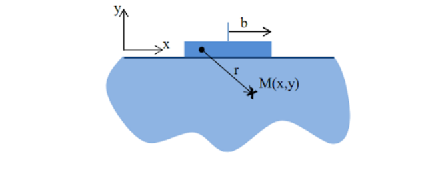
\includegraphics[scale=1]{../schéma et graphes/geo semi infni.png}
\captionof{figure}{Schema substrat semi fini}
\label{fig3}
\end{center}
La géométrie du problème ne se prêtant plus très bien à l’utilisation de coordonnées sphérique, on réalise un changement de variable pour repasser en coordonnées cartésiennes:
\begin{center}
$r=\sqrt{x^2+y^2}=x$
\end{center}
Pour finir, il est nécessaire de prendre en compte la largeur finie de l'élément chauffant:
\begin{center}
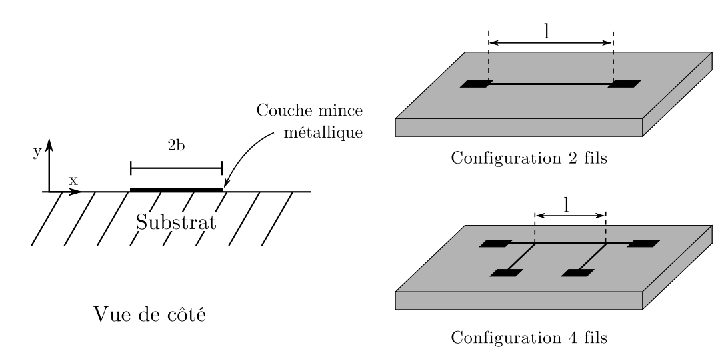
\includegraphics[scale=0.5]{../schéma et graphes/fil chauffant.png}
\captionof{figure}{Schema décrivant la géométrie des échantillons utilisés pour la méthode 3$\omega$}
\label{fig4}
\end{center}
Avec un produit de convolution, on obtient la variation de température en surface pour un fil de chauffe
\begin{center}
\begin{equation}
\Delta T_{ac}(w)=\frac{P_{rms}}{\pi\lambda l}\int_{0}^\infty \frac{sin^2(\eta b)}{(\eta b)^2\sqrt{q^2\omega+\eta^2}}d\eta
\end{equation}
où $\eta$ correspond au nombre d'onde (répétance c'est à dire la norme du vecteur d'onde)
\end{center}
Lorsque $\lvert qr<<1 \rvert$, avec un développement limité, on a:
\begin{center}
\begin{equation}
\Delta T_{ac}(\omega)=\frac{P_{rms}}{2\pi\lambda l}(ln(2\omega)+ln(b^2/D-2\epsilon)-i\frac{P_{rms}}{4\pi\lambda l}
\end{equation}
où $\epsilon$ est une constante d'ajustement approximativement égale à 0,922
\end{center}
\subsection{Calcul de la solution éxacte }
 Avec un changement de variable, on se ramène à l’intégrale suivante:
\begin{center}
\begin{equation}
\Delta T_{ac}=\frac{P}{\pi\Lambda}\int_{0}^\infty \frac{sin^2(y)}{y^2\sqrt{y^2+i\Omega}}dy
\end{equation}
avec $\Lambda=l\lambda$ et $\Omega=\frac{b^2\omega}{D}$
\end{center}
Cette intégrale peut alors être réécrite à l’aide des fonctions de Bessel et de Struve grâce à la relation suivante qui dérive d’une relation de récurrence sur les fonctions de Bessel. On désigne toujours par $K_{n}$ la fonction de Bessel à l’ordre n de deuxième espèce et par $L_{n}$ la fonction de Struve à l’ordre n:
\begin{center}
\begin{equation}
\int K_{0}(z)dz=\frac{z\pi}{2}[K_{0}(z)L_{-1}(z)+K_{1}(z)L_{0}(z)]=\frac{z\pi}{2}.f(z)
\end{equation}
\end{center}
En posant X=x/b la coordonées réduite, on obtient :
\begin{center}
\begin{equation}
T(x)=\frac{P}{4\Lambda}[(1-x).f(\sqrt{i\Omega(1-x)^2})+(1+x).f(\sqrt{i\Omega(1+x)^2})]
\end{equation}
\end{center}
\begin{center}
\end{center}
On peut également se ramener à une expression analytique à l’aide de la fonction de Meiger G:
\begin{center}
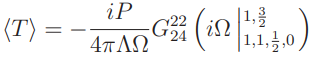
\includegraphics[scale=1]{../schéma et graphes/meijergbis.png}
\end{center}
avec la fonction de Meijer G définie comme tel:
\begin{center}
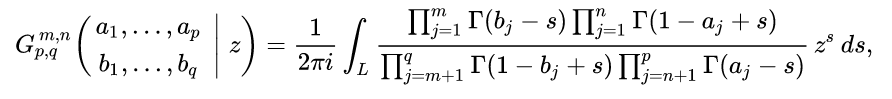
\includegraphics[scale=0.8]{../schéma et graphes/def_meijerg.png}
\end{center}
\chapter{Détermination numérique de la conductivité thermique }
Dans toutes cette partie, il s'agit de tracer numériquement l'amplitude de l'onde thermique en fonction de la fréquence afin d'en déduire la conductivité thermique.
\section{Régime linéaire: substrat seul}
Pour rappel,lorsque $\lvert qr<<1 \rvert$, avec un développement limité, on a:
\begin{center}
\begin{equation}
\Delta T_{ac}(w)=\frac{P_{rms}}{2\pi\lambda l}(ln(2\omega)+ln(b^2/D-2\epsilon)-i\frac{P_{rms}}{4\pi\lambda l}
\end{equation}
où $\epsilon$ est une constante d'ajustement approximativement égale à 0,922
\end{center}
La conductivité thermique est directement accessible d'une part via la pente de la courbe $T_{ac,x}(\omega)$ en fonction de $ln(2\omega)$ ou d'autre part grâce à $T_{ac,y}(\omega)$ supposée constante dans la gamme de fréquence du régime linéaire. Ce régime est obtenu soit pour des basses fréquences en raisonnant en fréquence , soit pour de petites largeurs de fil de chauffe en termes de géométrie.
\newline
\newline
Le tracé de la partie en quadrature de phase permet de s'assurer de la cohérence de ce que l'on trace car on sait qu'elle doit être constante quelque-soit la fréquence.
\begin{center}
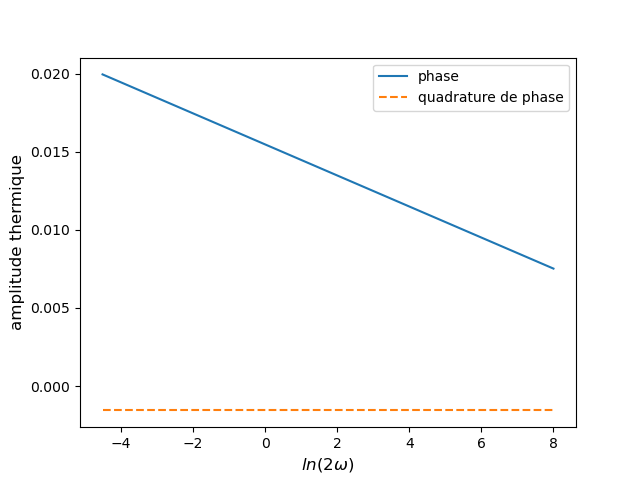
\includegraphics[scale=0.6]{../schéma et graphes/graphe_linéaire.png}
\captionof{figure}{Composantes de l'onde thermique en phase et en quadrature de phase en régime linéaire}
\end{center}
Pour déterminer la valeur de la conductivité thermique, deux méthodes s'offrent alors:
\newline
\newline
La première consiste à déterminer la pente k de la composante en phase. Elle permet alors de remonter à la valeur de la conductivité thermique:
\begin{equation}
k=\frac{P_{rms}}{2l\pi \lambda}
\end{equation}
\newline
La deuxième solution consiste à utiliser la composante en quadrature de phase. Dans le régime thermique linéaire, cette dernière est théoriquement constante et est inversement proportionnelle à la conductivité thermique :
\begin{equation}
T_{ac,y}=\frac{P_{rms}}{4\pi \lambda l}
\end{equation}
Néanmoins cette méthode n'est applicable que pour les basses fréquences ou les petites largeurs de fil de chauffe, d'où la nécessité d'utiliser la méthode 3$\omega$.
\newpage
\section{Régime non linéaire}
Le système étudié est alors le suivant:
\begin{center}
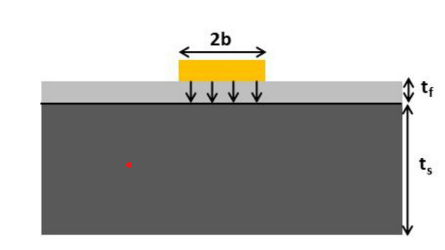
\includegraphics[scale=1]{../schéma et graphes/schema couches minces.png}
\captionof{figure}{système substrat et couches minces}
\end{center}
L'oscillation en température $\Delta T_{ac}$ s'écrit donc de la manière suivante:
\begin{center}
$\Delta T_{ac}=\Delta T_{f}+\Delta T_{s}$
\end{center}
Pour déterminer $k_{f}$ il s'agit de déterminer $\Delta T{f}$. En effet, lorsque $t_{f}<<2b$, l'onde de chaleur est une onde à une dimension se propageant dans la direction perpendiculaire au film mince. On a alors l'expression suivante:
\begin{equation}
\Delta T_{f}=\frac{P_{rms}t_{f}}{2bk_{f}}
\end{equation}
Par ailleurs, on obtient la valeur de $\Delta T_{ac}$ en mesurant le troisième harmonique de la tension (equation 3.10).
De plus, ayant déterminer la valeur $k_{s}$ du substrat dans la partie précédente, on remonte à la valeur de $\Delta T_{s}$ par la formule de Cahil (equation 4.1). On en déduit alors la valeur de $\Delta T_{f}$ puis la valeur de $k_{f}$:
\begin{equation}
k_{f}=\frac{P_{rms}t_{f}}{2b\Delta T_{f}}
\end{equation}
\begin{center}
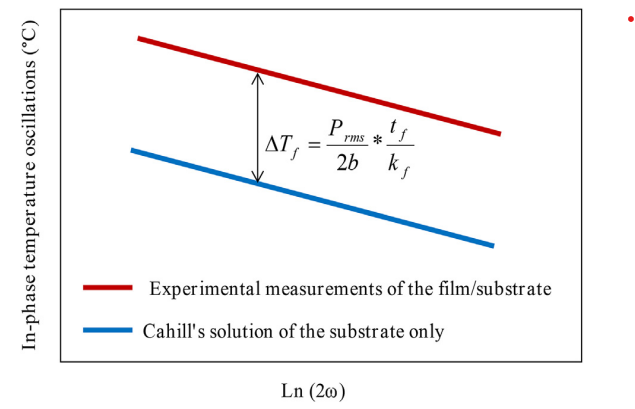
\includegraphics[scale=1]{../schéma et graphes/resiatnce.png}
\captionof{figure}{évaluation de Kf}
\end{center}
Pour tracer numériquement les oscillations de température, on utilise l'expression analytique trouvée en 3.3.2
En effet, on ne suppose plus ici que $\lvert qr\rvert<<1$. Il s'agit donc d'utiliser l'expression analytique générale des oscillations de l'onde de température trouvée dans la partie précédente:
\begin{center}
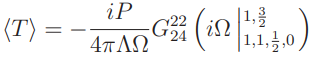
\includegraphics[scale=1]{../schéma et graphes/meijergbis.png}
\end{center}
On évalue alors tout d'abord la fonction de Meijerg comme une combinaison linéaire de séries hypergéométriques. Sous python, la fonction meijer g de la bibliothèque mp maths réalise cette évaluation. Une fois cette valeur calculée pour chaque valeur de fréquences, il ne reste plus qu'a calculer l'expression de l'oscillation en température à l'aide de la formule ci dessus. La quantité obtenue est donc un nombre complexe dont le module correspond à la composante en phase et l'argument à la composante en quadrature de phase.
\begin{center}
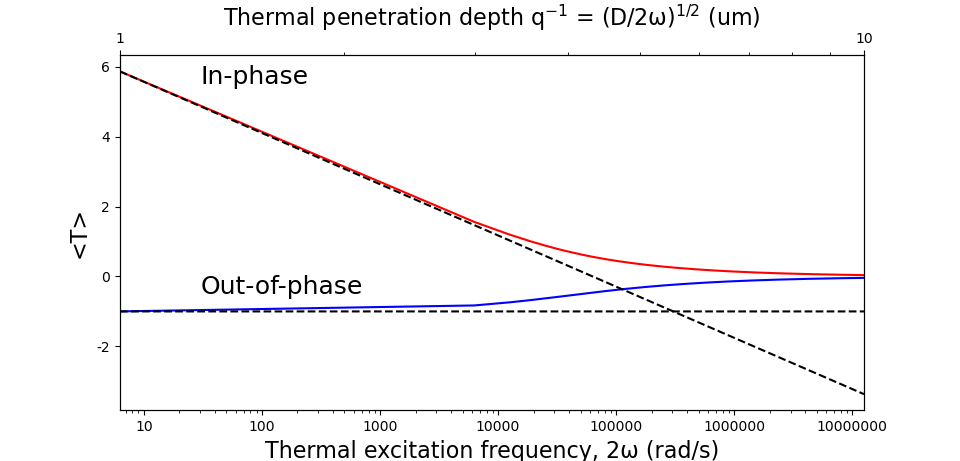
\includegraphics[scale=0.5]{../schéma et graphes/graphe_partie_nonlineaire.png}
\captionof{figure}{Composantes en phase et en quadrature de phase en régime non linéaire}
\end{center}
On trace de plus les composantes de la partie linéaire en pointillés pour s'assurer que nos tracés soit cohérent avec les résultats de la partie précédente.

\section{Résultats et Conclusions}
\subsection{Tracer des variations de température}
Il s'agit de regarder ici, à partir d'une conductivité thermique connue la cohérence du tracer à l'aide de la fonction de Meijerg.
Pour ce faire, on fait varier différentes grandeurs du modèle
\subsubsection{Influence de la largeur de l'élément chauffant}
\begin{center}
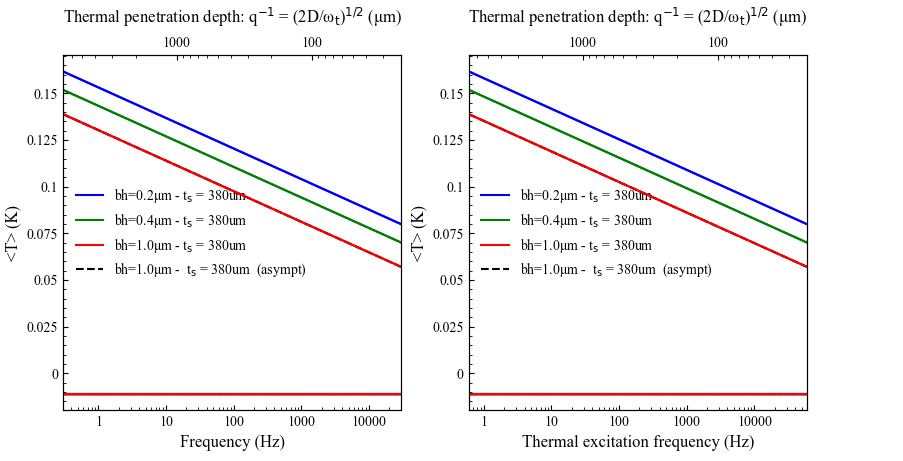
\includegraphics[scale=0.7]{../schéma et graphes/graphes1.png} 
\captionof{figure}{Variation de température pour différente valeur de largeur}
\end{center}
On voit clairement que plus la largeur de l'élément chauffant est grande, plus la variation de température est faible. Cela est cohérent puisque pour une même tension injectée dans l'élément chauffant, l'énergie dissipée par celui ci sera la même mais sur une surface d'autant plus grande que bh est grand. Donc, la puissance par unité de longueur est d'autant plus faible que bh est grand d'où l'observation.
\begin{center}
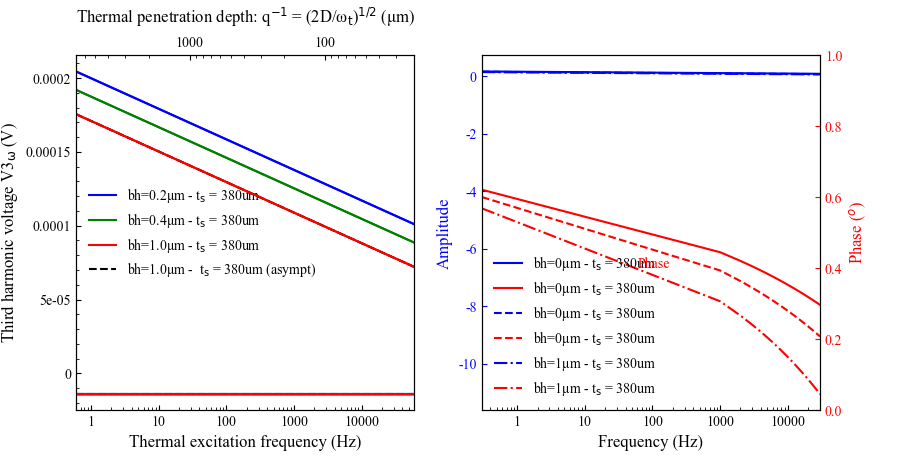
\includegraphics[scale=0.7]{../schéma et graphes/graphe2.png}
\captionof{figure}{Variation de la phase et de l'amplitude de l'onde} 
\end{center}
Au niveau de la phase et de l'amplitude de l'onde, encore une fois le tracé est cohérent puisque la phase diminue lorsque la largeur augmente. En effet, la puissance dissipée par unité de longueur étant plus faible, cela induit un déphasage au niveau de l'onde (elle mettra plus de temps à atteindre un point donné si elle l'atteint).
\subsubsection{Influence de la tension}
On réalise les même tracés que précédemment mais pour $V_{0}=2V$ (au lieu de $V_{0}=1V$)
\begin{center}
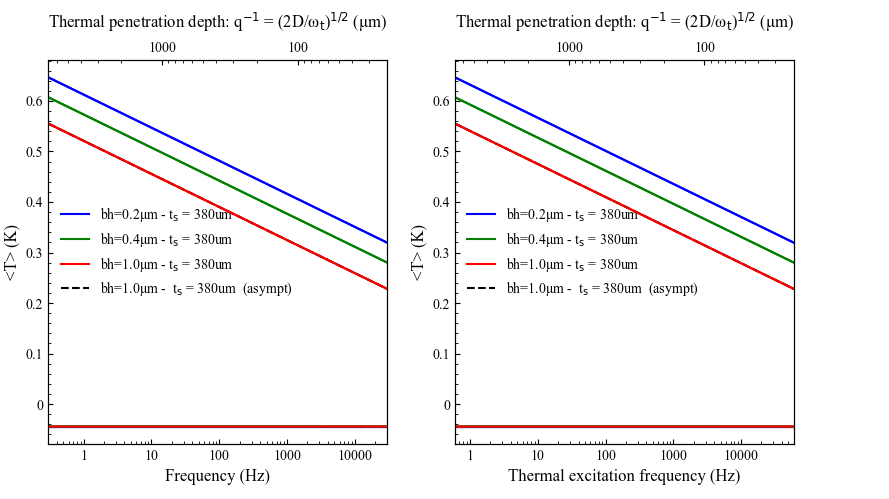
\includegraphics[scale=0.7]{influence_V0.png}  
\captionof{figure}{Variation de température pour V0=2V}
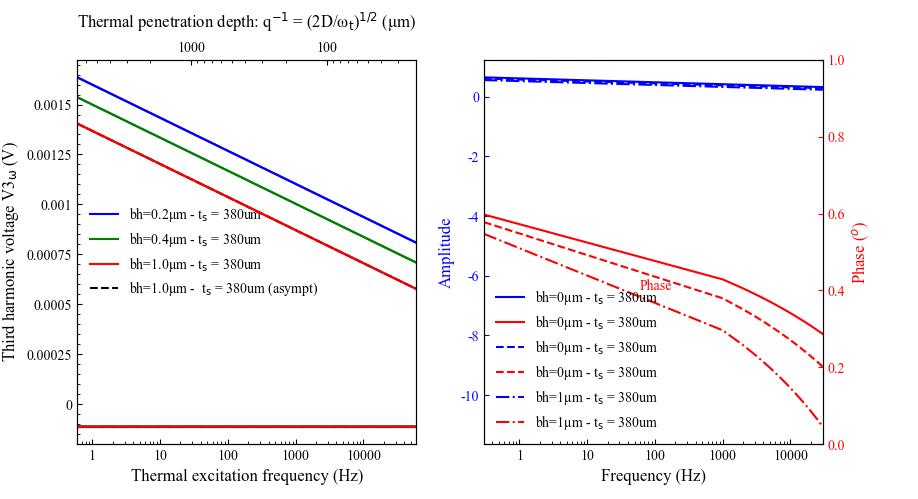
\includegraphics[scale=0.7]{influence_phaseV0.png}  
\captionof{figure}{Variation de la phase et de l'amplitude}
\end{center}
Pour une tension dont le fondamental est plus important, la puissance dissipée seras également plus importante ce qui explique que les variations de température observée pour $V_{0}=2V$ sont plus importante que pour $V_{0}=1V$. De même pour la phase et la valeur du troisième harmonique. 
\subsection{Calcul de la conductivité thermique du SiN}
Afin d'appliquer le raisonnement explicité de la section 4.2, il s'agit de tracer les variations de la composante en phase de la température pour le substrat seul et l'ensemble substrat-couche mince à partir des données expérimentales. Pour cela, ces données (fréquence, troisième harmonique, ...etc) sont stockées dans un fichier excel. 
\newline
Ensuite, à l'aide de la formule de Cahill, on trace les variations de la température du substrat seul grâce aux valeurs de fréquences stockées dans le fichier excel. De même, on remonte à la valeur de $\Delta T_{ac}$ grâce aux valeurs du troisième harmonique stockées dans ce même fichier.
\subsubsection{Pour un film d'une épaisseur de 100 nm}
\begin{center}
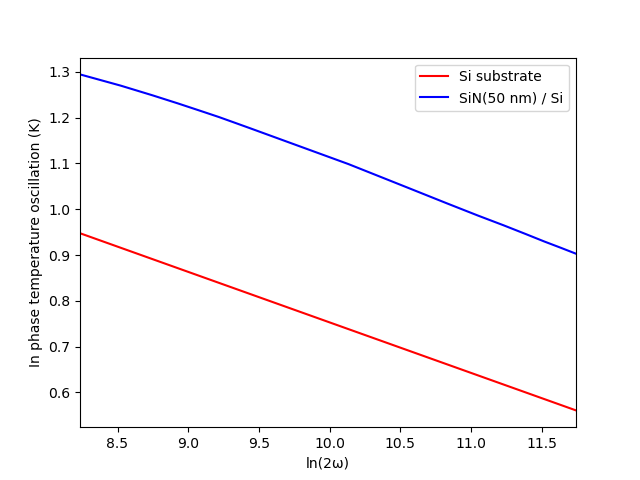
\includegraphics[scale=0.7]{50nm.png}
\captionof{figure}{Variation de température pour Si(substrat) et Si + film}
\end{center}
\subsubsection{Pour un film d'une épaisseur de 100nm}
\begin{center}
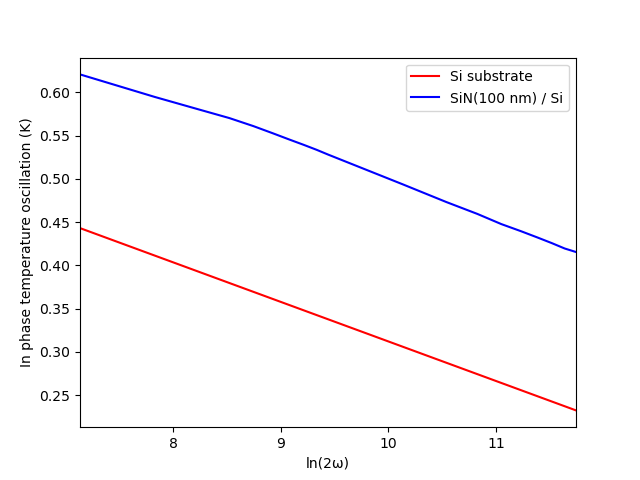
\includegraphics[scale=0.7]{100nm.png} 
\captionof{figure}{Variation de température Si(substrat) et Si + film}
\end{center}
Les valeurs  de température (celles du substrat seul et les partie réelle et partie imaginaire de l'ensemble couche-mince-substrat) calculées pour chaque fréquences sont alors stockées dans une dataframe. On créer de plus deux champs supplémentaires dans lesquels seront stockées les valeurs de température du film et de conductivité calculées par la suite.
\newline
On calcul ensuite de le $\Delta T_{f}$ en faisant la différence entre les deux variations de température calculées et on stocke ces valeurs dans la dataframe. On en déduit alors la valeur de la conductivité du film grâce à la formule 4.5 que l'on stocke également dans la data frame.
\subsubsection{Pour un film d'épaisseur de 50nm}
\begin{center}
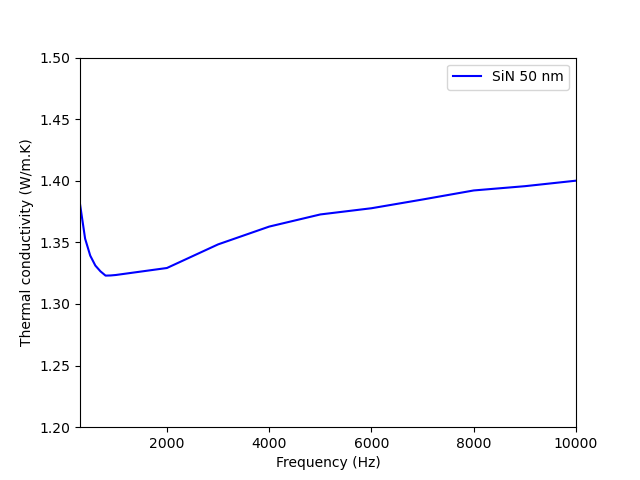
\includegraphics[scale=0.7]{kappa50nm.png} 
\captionof{figure}{valeurs de $k_{f}$ }
\end{center}
\subsubsection{Pour un film d'épaisseur de 100nm}
\begin{center}
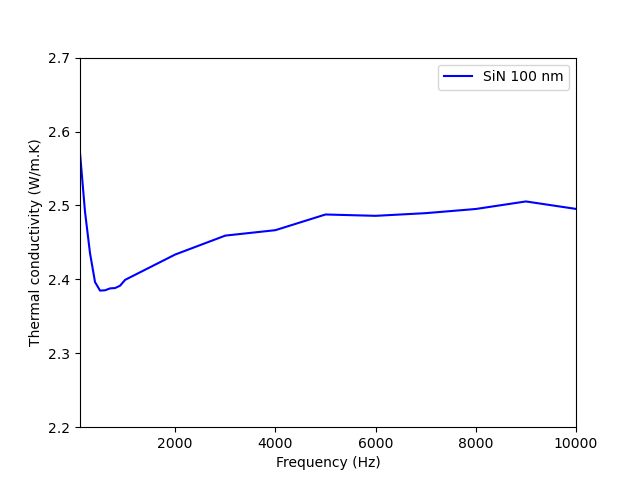
\includegraphics[scale=0.7]{kappa100nm.png} 
\captionof{figure}{valeurs de $k_{f}$}
\end{center}
On obtient un $k_{f}$ moyen de 1,35 W/(m.K) pour la couche à 50 nm et de 2,45 W/(m.K) pour la couche de 100nm.
\newline
\newline
Tout d'abord les valeurs trouvées sont cohérentes avec l'expression de la profondeur de pénétration. En effet, celle ci dépend de la fréquence d'excitation et plus la fréquence est faible (pour une diffusivité fixée) plus elle est faible. Cette grandeur représentant l'épaisseur sur laquelle l'onde thermique se diffuse, il est donc logique d'avoir une conductivité plus forte à haute fréquence qu'à basse fréquence.

De plus, les valeurs moyennes trouvées son cohérentes avec celles de la littérature: 1.34 W/(m.K)
\section{Répartition du travail de groupe}
Malgré qu'il soit souvent difficile dans ce type de projet de compartimenter le travail, nous nous sommes efforcé d'essayer de le faire. Nous avons tout d'abord pris le temps de bien comprendre le modèle utilisé tous ensemble. Ensuite, nous avons tous ensemble travailler sur chaque étape du projet. Chaque membre expliquait aux autres ce qu'il avait compris et proposait des raisonnements sur les résultats que l'on obtenait.
\begin{thebibliography}
D G. Cahill and R. O. Pohl, “Thermal conductivity of amorphous solids above the plateau,” Physical Review B,
vol. 35, no. 8, pp. 4067–4073, 1987.
\newline
\newline
J-Y. Duquesne, D. Fournier, and C. Frétigny, “Analytical solutions of the heat diffusion equation for 3$\omega$ method
geometry,” Journal of Applied Physics, vol. 108, no. 8, p. 086104, 2010.
\newline
\newline
 W. Jaber and P.-O. Chapuis, “Non-idealities in the 3$\omega$ method for thermal characterization in the low- and high-
frequency regimes,” AIP Advances, vol. 8, no. 4, p. 045111, 2018.
\newline
\newline
A. A. Guermoudi, P. Y. Cresson, A. Ouldabbes, G. Boussatour, and T. Lasri, “Thermal conductivity and
interfacial effect of parylene C thin film using the 3-omega method,” Journal of Thermal Analysis and
Calorimetry, 2020.
\newline
\newline
G. Boussatoura , P-Y Cressona, B Genestie, N Joly, J.F Brund, T Lasri, "Measurement of the thermal conductivity of flexible biosourced polymersusing the 3-omega method"
\newline
\newline
Emmanuel GIUDICELLI, Nadia MARTAJ, Rachid BENNACER , Y. CUMINAL1 et Philippe COMBETTE, "Caractérisation thermique des cellules photovoltaïques multi-jonction par la méthode 3$\omega$"
\newline
\newline
https://docs.sympy.org/latest/modules/integrals/g-functions.html
\newline
\newline
https://mpmath.org/doc/current/functions/hypergeometric.html
\newline
\newline
https://fr.wikipedia.org/wiki/Fonction-de-Bessel
\end{thebibliography}
\end{document}